\documentclass[12pt, a4paper]{article}
\input{preamble_GP_hw1}  % 使用自己維護的定義檔
%-----------------------------------------------------------------------------------------------------------------------
% 文章開始
\title{ \XeLaTeX {\KT 的各種表現技巧}}	% 使用設定的字型
\author{{\KT 林貫原}}				% 使用設定的小字體
\date{{\R \today }} 			
\begin{document}
\renewcommand{\tablename}{表}	
\renewcommand{\figurename}{圖}
\maketitle
\fontsize{12}{22pt}\selectfont 

\BB 區塊鏈技術在當今的數字時代嶄露頭角,它不僅是加密貨幣的基礎,還是分散式應用程序的基礎。其中,以太坊作為區塊鏈一個引人注目的實現,推動了分散式應用程序的發展,重新定義了數位世界的未來。區塊鏈,簡而言之,是一種分散式的數據庫技術,它記錄了交易和信息,並且這些記錄不可被篡改。它不僅在金融領域廣泛應用,還在供應鏈、醫療保健等領域發揮。而以太坊則是區塊鏈技術的一個巨大飛躍,它提供了更多靈活性和功能性。以太坊不僅支持以太幣,還能運行智能合約,這是一種自動執行的協議,無需中間人參與。這使以太坊成為分散式應用程序的首選平台。總之,區塊鏈和以太坊代表了去中心化的數字未來,它們改變我們對數據和交易的看法。隨著技術不斷演進,區塊鏈和以太坊將繼續在我們生活中扮演著越來越重要的角色,塑造著未來的分散式數字世界。
\section{\textit {\SK 何謂區塊鏈}}
區塊鏈是一種新穎的科技,就像是AI (Artificial intelligence)人工智慧,抑或是VR (Virtual Reality)虛擬實境,而比特幣就是第一個應用「區塊鏈」技術產生的貨幣。

\section{\textsl {\SK 特色}}

\subsection{\textbf {\SK 去中心化}}
\bigskip
	\begin{lstlisting}
有些人也會稱「去中介化」,意即無固定中心,為分散式結構。
	\end{lstlisting}
\bigskip
目前生活中大部分服務的運作方式都是中心化的,針對每件事有一個集中的管理中心負責處理各種事項。
舉個例子,大多數人會將積蓄存在銀行裡,而帳戶中每筆資料皆會被收集在該銀行的資料庫,比如說登錄網路銀行、帳戶餘額、匯款紀錄等等,且存入銀行的積蓄即轉變為銀行的資金,而此資金的動用權力全權掌握於該銀行中,比如說轉帳需要經過銀行的授權、若某人被檢察官查到有非法所得,則可運用公權力要求銀行凍結該帳戶。

這個鮮明的特性讓區塊鏈技術被稱作「分散式帳本技術」,也曾讓人認為去中心化的區塊鏈技術將會取代「銀行」的角色。
去中心化原理:如圖 \ref{fig:central} (a),每一個區塊就像帳本中的每一頁,上面記錄了許多交易的細節,例如小時候媽媽給你零用錢,想要存錢的你總是在自己的小本本上記帳。帳本技術到這裡沒有問題,但分散式呢?
如圖 \ref{fig:central} (b),分散式指的是區塊鏈系統中的每一位參與者,我們稱作節點,系統中所有的節點「共同維護與更新」同一本帳本,且每一個節點都會各自保留一份小備份,沒有中央伺服器來管理秩序。想像一下,如果你哥哥貪圖你的零用錢,跑去改掉你小本本上的紀錄,並且拿走你所有的零用錢,要是他的橡皮擦功力夠強,你根本抓不到痕跡吧?於是「分散式節點的備份」成為確保區塊鏈系統安全性的關鍵之一。
\begin{figure}[H]
    \centering
        \subfloat[中心化示意圖]{
        \includegraphics[scale=0.6]{\imgdir centralization.png}}
        \subfloat[去中心化示意圖]{
        \includegraphics[scale=0.6]{\imgdir decentralization.png}}
    \caption{有無中心組織示意圖}
    \label{fig:central}
\end{figure}
\subsection{\SM 匿名性}
「匿名性」是區塊鏈系統中的一項特性,允許節點以不具名的方式參與,每個節點都使用一組獨一無二的代碼(通常由英文字母和數字組成)作為其識別,只要這個代碼不被揭示,則無法追蹤到節點背後的真實身份。這種匿名性特性有時會引起人們對區塊鏈可能被用於洗錢等非法活動的擔憂,因此各國政府對區塊鏈技術和加密貨幣的監管都持謹慎態度,這也是其主要考慮因素之一。
\subsection{\PP 不可篡改}
\bigskip     %加大垂直行距美觀排版
\begin{center}\colorbox{bubbles}{\begin{tabular}{p{0.9\textwidth}}
	 {區塊鏈的資料都是公開的,可供任何人查閱。	}
\end{tabular}}
\end{center}
\bigskip	
帳本分散存儲在眾多參與者之間,每次更動必須經過多數同意,持續進行加密和驗證以確保安全,所有交易明細都在公開鏈上顯示。這與中心化體系不同,例如銀行的集中式資料庫,區塊鏈提供了更高程度的公開透明度,顯著降低了不透明操作的可能性。

每次更新必須經過驗證並獲得多數同意,因此無法單方面進行更動。已經被打包的交易經過加密處理,並且一旦上鏈,就無法被竄改。這正是區塊鏈的一項特性,即「不可篡改性」。

然而,這不表示區塊鏈是絕對無誤的。如果有人試圖掌握超過51\%的計算能力,則有可能出現各種交易錯誤和混亂。但要實現這樣的攻擊,難度和成本都非常高,特別是在參與者眾多的大規模區塊鏈網絡中。這種情況被稱為「51\% 攻擊」,攻擊者必須掌握多數算力\footnote {多數算力(majority of computing power)是指在區塊鏈網絡中,超過50\%的計算能力,通常由參與網絡的節點(如礦工或挖礦者)提供。這些節點在區塊鏈的共識機制中發揮關鍵作用,需要多數節點就提案或交易達成共識,以確保區塊鏈的安全性和一致性。如果某人掌握超過50\%的計算能力,他們將有能力主導整個區塊鏈網絡,可能修改交易或執行惡意操作。這種攻擊被稱為 "51\% 攻擊",然而,實施此類攻擊非常昂貴和困難,特別是在參與節點眾多且計算能力分散的大型區塊鏈網絡中,因此,大多數區塊鏈網絡都具有很高的安全性,成功攻擊的風險很低。}以控制區塊鏈運作,但愈大規模和去中心化的區塊鏈更難受到攻擊。

總之,參與者愈多,區塊鏈的規模愈大,其安全性愈高,這也強調了去中心化的重要性。
\subsection{\BB 講求共識}
區塊鏈技術中最顯著且最民主的機制莫過於「共識演算法」。每種區塊鏈系統都會採用特定的共識演算法。以比特幣區塊鏈為例,它使用的是「工作量證明」共識演算法。然而,這種共識演算法面臨的主要問題在於,當人們意識到工作量越大,挖掘比特幣的機會越高時,他們就會紛紛增加計算能力,包括使用更多的遊戲顯示卡(GPU)和中央處理器(CPU),甚至結合其他節點,以集中算力提高挖掘比特幣的機會,並以分紅方式分享獲利。這種行為常見的方式包括租借雲端計算能力和參與礦池。
\subsection{\WW 加密}
區塊鏈技術的加密性質在虛擬貨幣應用中發揮了關鍵作用,特別是在涉及「公鑰和私鑰」的情況下。這些特性應用於電子錢包、資產管理、驗證機制等領域,具體表現在以下方面:
\begin{itemize}
\item 個人資產管理:區塊鏈技術允許用戶擁有自己的數位資產,並使用私鑰來控制和管理這些資產。這意味著你可以完全自主地管理你的虛擬貨幣和資產,無需依賴中央機構或金融機構。
\item 信任問題的解決:區塊鏈的去中心化性質,以及公鑰和私鑰的加密機制,消除了人與人之間的信任問題。交易和合約的執行不再依賴於單一的中介機構,而是基於數學和加密技術,使得交易更加安全且可靠。
\item 安全性提升:公鑰和私鑰的組合提供了高度的安全性。私鑰只有擁有者可以訪問,並用於簽署交易,確保只有合法的所有者可以進行交易。這樣的安全性使虛擬貨幣和資產受到保護,減少了盜竊和欺詐的風險。
\item 交易效率提高:區塊鏈技術通常允許快速、全天候的交易,而不受地理位置或時間的限制。這提高了交易效率,使人們能夠更快速地完成金融交易和跨境支付。
\end{itemize}
總之,區塊鏈的加密性質以及公鑰和私鑰的應用為虛擬貨幣和區塊鏈生態系統帶來了許多優勢,包括安全性、信任、個人資產管理和交易效率的提升。這些特性正在不斷推動區塊鏈技術的應用擴展到更多領域。
\vspace{0.5cm}
\begin{figure}[h]
    \centering{
        \includegraphics[scale=0.3]{\imgdir five-characteristic .jpeg}}
    \caption{五大特色圖}
    \label{fig:five-characteristic}
\end{figure}

\begin{table}[H]
\centering
    \caption{區塊鏈特色比較} \label{tb:區塊鏈特色比較}
    \renewcommand{\arraystretch}{2}
%    \extrarowheight=1.5pt
\begin{tabular}{|c|c|c|}
\hline
\cellcolor{lightgray}{\backslashbox{\textbf{特色}}{\textbf{優缺}}} & \cellcolor{bubbles}{優點} & \cellcolor{bubbles}{缺點} \\
\hline
\cellcolor{mistyrose}{去中心化} & \cellcolor{cream}{抗攻擊性} & \cellcolor{cream}{效率較低} \\
\hline
\cellcolor{mistyrose}{不可篡改} & \cellcolor{cream}{隱私保護} & \cellcolor{cream}{潛在濫用} \\
\hline
\cellcolor{mistyrose}{講求共識} & \cellcolor{cream}{信任建立} & \cellcolor{cream}{錯誤難修正} \\
\hline
\cellcolor{mistyrose}{匿名性} & \cellcolor{cream}{安全可靠} & \cellcolor{cream}{複雜性增加} \\
\hline
\cellcolor{mistyrose}{加密} & \cellcolor{cream}{資料保密} & \cellcolor{cream}{密鑰管理需謹慎} \\
\hline
\end{tabular}
\end{table}
\section{比特幣(bitcoin)}
\begin{figure}[H]
    \centering
    \subfloat[bitcoin1]{
        \includegraphics[scale=0.35, angle=30, width=6cm, height=2cm]{\imgdir bitcoinnnn.png}
    }
    \subfloat[bitcoin2]{
        \includegraphics[scale=0.35, angle=330, width=6cm, height=2cm]{\imgdir bitcoinnnn.png}
    }
    \caption{BTC}
    \label{fig:bitcoinnnn}
\end{figure}
比特幣(Bitcoin,縮寫:BTC 或 XBT)是一種基於去中心化,採用點對點網路與共識主動性,開放原始碼,以區塊鏈作為底層技術的加密貨幣,比特幣由中本聰(網名)(Satoshi Nakamoto)於2008年發表論文,2009創世區塊誕生。在某些國家、央行、政府機關、學術界則將比特幣視為虛擬商品,而不認為是貨幣。貨幣金融學認為貨幣具有交易媒介、記賬單位、價值儲藏和延期支付四種基本職能,但由於其高度波動性因此不具有後兩種基本職能從而不是貨幣。
\begin{SCfigure}[0.9][h]  % 數字 0.9 代表圖形開始的位置
\caption{比特幣}
\includegraphics[width=0.4\textwidth]{\imgdir goldbitcoin.jpeg}
\label{fig:bitcoinn}
\end{SCfigure}

\section{以太幣(\textbf{ETH})}
\begin{wrapfigure}{R}{0.4\textwidth}
\centering
\includegraphics[width=0.4\textwidth]{\imgdir eth.jpeg}
\newpage
\caption{以太幣}\label{fig:eth}
\end{wrapfigure}
以太幣(Ether,縮寫ETH),以太幣(ETH)是一種虛擬貨幣(加密貨幣),是以太坊的基礎貨幣,可以用在以太坊的產品或是服務上付款,包括交易時所發生的手續費用,以及運行智能合約、或者因為採礦所得到的獎勵等等,而以太幣就是可以在以太坊所開發的區塊鏈平台中能進行交易的一種加密貨幣。 

以太幣(ETH)採用與比特幣不同的區塊鏈技術,主要使用在以太坊(Ethereum)區塊鏈上。不同於比特幣總發行量為2,100萬枚,而以太幣(ETH)在發行數量上不設限,是僅次於比特幣之後第二高發行量的加密貨幣。
\subsection{以太坊(\textsl{Ethereum})}
以太坊(Ethereum)是一個為全球提供開源的公共區塊鏈技術平台,與其他區塊鏈網路的差異就是多了智能合約與DApp技術。以太坊的目的是創造一個去中心化的世界電腦,協助去中心化的應用程式免受政府審查和遭受篡改的影響。 

而以太坊的核心技術是以太坊虛擬機Ethereum Virtual Machine(EVM),它可以執行高度複雜的演算法代碼。技術人員透過JavaScript和Python等程式語言為模型,編寫成在以太坊虛擬機(EVM)上運行的應用程序,稱為「DApp」。
\subsection{礦工}
以太坊為了安全有兩個驗證機制,第一個驗證就是要拿公開的鑰匙插進訊息中的鎖頭,確認是否可以被解開,如果有人冒名發送訊息,那就會解不開訊息裡的鎖頭,而知道這是假冒的交易資訊,確認是本人發送後,帳戶餘額足夠進行交易,就能交易成功,接著這筆交易訊息就會被放進一個新生成的資訊塊中,這部分後頭介紹公鑰與私鑰會做說明。\\
至於第二個驗證機制就是在每個資訊塊的末端會再放進另一組驗證碼,而這個驗證碼會被錄製到下一個資訊塊裏面,下一塊的驗證碼就會被放進到下下個資訊塊中,用環環相扣的驗證碼來確認區塊鏈沒有被任意竄改,好處是若區塊鏈被動了手腳,就會導致驗證編碼前後不一致,進而宣告此資訊塊不可信,這也是為何區塊鏈公開透明卻不會被任意改寫的原因,不過要驗證鑰匙和鎖頭是否相合或是驗算這個新資訊塊的前後驗證碼是否正確都是一件相當累人的事,所以系統會設計願意提供計算能力的人一些獎勵,以以太幣來說,算最快的人就會有POW,就是上頭的工作量證明,有了這個證明就會獲得一些額外的以太幣,而這種幫忙驗算的動作就叫做挖礦,而這些人就叫做礦工。

\begin{figure}[h]
    \centering{
        \includegraphics[scale=0.3]{\imgdir 區塊鏈1.png}}
    \caption{區塊鏈驗證}
    \label{fig:區塊鏈驗證}
\end{figure}
\begin{figure}[h]
    \centering{
        \includegraphics[scale=0.3]{\imgdir 區塊鏈2.png}}
    \caption{區塊鏈驗證過程}
    \label{fig:區塊鏈驗證過程}
\end{figure}
\subsection{Gas}
以太坊的燃料稱作Gas,有點交易手續費的概念,所以只要經過任何的運算,都需要繳交些許的Gas,包括發送一些以太幣或其他代幣,代幣也被稱作Tokens,每次交易發送方都需要設置一個Gas Limit與Gas Price,Gas Limit是指你最高願意付出多少Gas,而Gas Price就是你每個Gas要付出多少的Ether,他是用Gwei來計算,而一個以太幣是10的18次方Wei,一個Gwei是10的9次方wei,簡單舉個例子,假設現在設定的Gas Limit是10000,Gas Price是10Gwei,那發送方願意為此交易付出的最大金額就是兩者相乘,也就是10的負4次方,也就等於0.0001個Ether。
\begin{table}[h]
\begin{center}
\caption{Gas介紹}\label{tb:Gas}
\extrarowheight=4pt
\begin{tabular}{ll}
\rowcolor[gray]{.9}
名詞			&	說明\\
\toprule
Gas Limit	&	最高願意付出多少Gas\\
Gas Price	&	每個Gas要付出多少的Ether\\
Wei      	&	以太坊中最小的計算單位\\
Gwei      	&	以太坊中的一個單位$1Gwei=10^9wei$\\
Tokens	    &	代幣,$1Ether=10^{18}wei$\\
\bottomrule
\end{tabular}
\end{center}
\vspace{1cm}
\end{table}
\begin{longtable}{@{}lrr@{}}
\caption{Gas Limit Price}
\label{tb:Gaslimitprice}\\
\toprule
Gas Limit& Gas Price& 最高金額\\
\midrule
\endfirsthead
\multicolumn{3}{l}{承接上頁}\\[2pt]
\toprule
Gas Limit& Gas Price& 最高金額\\
\midrule
\endhead
\midrule
\multicolumn{3}{r}{續接下頁}
\endfoot
\endlastfoot
100     &1000Gwei    &0.0001Ether\\
1000    &100Gwei     &0.0001Ether\\
10000   &10Gwei      &0.0001Ether\\
100000  &1Gwei       &0.0001Ether\\
100     &10000Gwei   &0.001Ether\\
1000    &100000Gwei  &0.1Ether\\
10000   &1000000Gwei &10Ether\\
50      &2000Gwei    &0.0001Ether\\
500     &2000Gwei    &0.001Ether\\
5000    &200Gwei     &0.001Ether\\
50000   &20Gwei      &0.001Ether\\
20      &5000Gwei    &0.0001Ether\\
200     &50000Gwei   &0.01Ether\\
2000    &500000Gwei  &1Ether\\
20000   &5000000Gwei &100Ether\\
2500    &4Gwei       &0.00001Ether\\
2500    &40Gwei      &0.0001Ether\\
2500    &400Gwei     &0.001Ether\\
2500    &4000Gwei    &0.01Ether\\
2500    &40000Gwei   &0.1Ether\\
40      &250Gwei     &0.00001Ether\\
400     &250Gwei     &0.0001Ether\\
4000    &250Gwei     &0.001Ether\\
40000   &250Gwei     &0.01Ether\\
400000  &250Gwei     &0.1Ether\\
40      &2500Gwei    &0.0001Ether\\
400     &2500Gwei    &0.001Ether\\
4000    &2500Gwei    &0.01Ether\\
40000   &2500Gwei    &0.1Ether\\
400000  &2500Gwei    &1Ether\\
80      &12500Gwei   &0.001Ether\\
800     &12500Gwei   &0.01Ether\\
8000    &12500Gwei   &0.1Ether\\
80000   &12500Gwei   &1Ether\\
800000  &12500Gwei   &10Ether\\
125     &800Gwei     &0.0001Ether\\
1250    &800Gwei     &0.001Ether\\
12500   &800Gwei     &0.01Ether\\
125000  &800Gwei     &0.1Ether\\
1250000 &800Gwei     &1Ether\\
125     &400Gwei     &0.00005Ether\\
1250    &400Gwei     &0.0005Ether\\
12500   &400Gwei     &0.005Ether\\
125000  &400Gwei     &0.05Ether\\
1250000 &400Gwei     &0.5Ether\\
12500   &200Gwei     &0.0025Ether\\
125000  &200Gwei     &0.025Ether\\
1250000 &200Gwei     &0.25Ether\\
\bottomrule
\end{longtable}
通常這些Gas會被發送到礦工的帳戶地址,就是剛剛說的驗證這筆交易的人的獎勵,所以如果發送方願意支付的Gas價格越高,礦工所獲得的價值就越多,因此會有更多或比較厲害的礦工優先選擇他,因為礦工是可以選擇要驗證哪些交易或忽略哪些交易的。至於GAS發送有下面兩種狀況:\\
\begin{figure}[H]
    \centering{
        \includegraphics[scale=0.55]{\imgdir Gas1.png}}
    \caption{Gas Enough}
    \label{fig:Gasenough}
\end{figure}
第一種是如果發送方帳戶裡有足夠的Ether,交易結束時如果Gas沒有花完就會退還給發送方。\\
\begin{figure}[H]
    \centering{
        \includegraphics[scale=0.55]{\imgdir Gas2.png}}
    \caption{Gas not enough}
    \label{fig:Gasnotenough}
\end{figure}
第二種狀況的話,是如果發送方的帳戶不能提供足夠的Ether,那交易的時候就會有餘額不足的情形,那就會導致半路就沒有辦法繼續下去,所以這筆交易會判定為無效的,而過程因為也有經過運算所以消耗的Gas也不會退還。
\subsection{Forks}
全世界的礦工一起工作如果狀態不一致,就可能倒置產生很多鏈出來,這就是所謂的分叉。因為區塊鏈都是共享的狀態,所以分叉會破壞到系統,所以為了防止這種分叉的狀況,以太坊使用一種GHOST協議,這個協議就是告訴大家,如果發生了這種狀況的話,必須選擇鏈上計算最多的路徑,最簡單的方法就是計算路徑上的區塊數量,但不計算初始的區塊,數量越多的話代表路徑越長,挖礦的難度就會越大。分叉其實還有分成軟分叉跟硬分叉,硬分叉的話是因為網路延遲,產生兩個區塊來,但隨著時間走,等待下一個區塊的產生,區塊鏈就會收斂正常了,軟區塊就比較不一樣,是因為共識機制的改變,未更新共識機制的人會照著原本的區塊走,比如說今天捷運公司宣佈只有穿西裝的人才可以搭板南線,但沒穿西裝的人依舊可以搭其他的路線,所以說沒有更新的版本的節點只是不能參與新的共識機制,但依舊可以兼容某些情形。
\vspace{0.5cm}
\begin{figure}[h]
    \centering{
        \includegraphics[scale=0.65]{\imgdir Forks.png}}
    \caption{Forks}
    \label{fig:Forks}
\end{figure}
\subsection{私鑰公鑰地址}
\begin{enumerate}
\item 私鑰:
以太坊的私鑰是一串隨機生成的256bits,也就是說有2的256次方種可能,所以要生成兩個一模一樣的私鑰是一件幾乎不可能發生的事。私鑰可以簽署交易,就像在現實生活中需要簽名才能夠轉帳一樣,簽署過後的交易才能夠對你的帳戶資產進行更改。所以雖然在區塊鏈中大家都可以產生一筆交易更動你的資產,但是只有擁有私鑰的人才能夠簽署這筆交易,交易才能被認可和被驗證。在現實世界中可以捏造一個假的簽名,完成交易,但是在區塊鏈的世界中,因為它底層的密碼學特性,這件事情是不可能發生的,目前沒有一個人可以在沒有私鑰的情況下簽署交易。不過要小心的是如果有人知道你的私鑰,那麼他就擁有你所有的資產了,所以一定邀將自己的私鑰保管好。
\item 公鑰:
在以太坊中,私鑰是用來將訊息簽名的,而公鑰是用來驗證簽名的,所有人都可以獲取你的公鑰以驗證簽名。先講一下單向函數,就是輸入一個input到函數$f(x)$,會很容易地得到output,但是只給定output卻很難反向計算出input。以太坊的公鑰是由私鑰經過橢圓曲線數字簽名演算法算出來的,得出的結果長度為512 bits,其演算法使用橢圓曲線這個單向函數。因此透過私鑰轉換成公鑰非常容易,但是要透過公鑰轉換成私鑰是一件非常困難的事,這也恰恰符合前面所說的私鑰不能隨意洩露。
\item 地址:
地址就像銀行帳號,是以太坊中用來代表一個帳戶的方式,任何交易都是由一個地址發起的,以太坊的地址是由公鑰生成的,先將公鑰代入函數中,這個函也數是一個單向函數,其output長度為256 bits,Ethereum 取最右邊的160 bits作為帳戶地址,所以地址有2的160次方種可能。 
\end{enumerate}
\begin{figure}[h]
    \centering{
        \includegraphics[scale=0.6]{\imgdir 私鑰公鑰地址.png}}
    \caption{私鑰公鑰地址}
    \label{fig:pkpkadd}
\end{figure}
用圖 \ref{pkpkadd} 簡單講一下剛剛的概念,私鑰經過橢圓曲線數字簽名演算法生成公鑰,而公鑰再經過雜湊函數生成地址(256bits取右側160bits)。
\begin{figure}[H]
    \centering{
        \includegraphics[scale=0.7]{\imgdir 公私鑰示意圖1.png}}
    \caption{公私鑰示意圖狀況1}
    \label{fig:keysituation1}
\end{figure}
圖 \ref{keysituation1} 為公鑰加密,私鑰解密:為了保護訊息本身,用接收訊息者的公鑰加密,只有對方的私鑰可以開啟訊息\\
舉例:我要傳送一筆重要資料或訊息給學長,所以我用學長的公鑰加密,由於私鑰生成公鑰,公私鑰成對的原理,所以只有學長的私鑰可以開啟這份資料。\\
\begin{figure}[H]
    \centering{
        \includegraphics[scale=0.7]{\imgdir 公私鑰示意圖2.png}}
    \caption{公私鑰示意圖狀況2}
    \label{fig:keysituation2}
\end{figure}
圖 \ref{keysituation2} 為私鑰加密,公鑰解密:為了證明所發出的資料或訊息是發布者本人(也就是私鑰持有者)。\\
舉例:我今天要以我的名義公告一件事,但是要如何確定這是我本人要發佈的呢?所以我就得用我的私鑰加密這則訊息,這個行為就像是數位簽章(Digital Signing),然後因為我的公鑰是可以公開的,所以想知道這則訊息的人,只要用我的公鑰來解密。\\
\subsection{雜湊函數(Hash Function)}
現在最夯的虛擬貨幣,使用的是區塊鏈的原理,而區塊鏈就是使用雜湊函數進行運算,像比特幣選擇的是SHA-256,而以太幣是Keccak(SHA-3)。
Hash Function是一種數學函數,它將任意長度的輸入訊息(或數據)轉換為固定長度的二進制數字串,這個固定長度通常稱為散列值(Hash Value)或摘要(Digest)。這個轉換過程是單向的,意味著很難從散列值中還原出原始輸入。以下是他的四大特性:
\begin{enumerate}
\item 固定輸出長度:不論輸入訊息有多長,雜湊函數的輸出始終具有相同的固定長度。例如,SHA-256的散列值始終是256位(32位元組)。
\item 唯一性:每個不同的輸入應該產生不同的散列值。即使輸入的訊息只有微小的改變,也應該導致完全不同的散列值。這種性質被稱為「無碰撞性」。
\item 效能好:計算雜湊函數的散列值應該在合理的時間內完成,即使對於大型輸入也是如此。
\item 不可逆性:從散列值應該極難或幾乎不可能還原出原始輸入。這是雜湊函數的關鍵特點之一。
\end{enumerate}
至於要怎麼去比對使用者輸入的值是不是正確的?只要在使用者輸入密碼後,去進行雜湊,再和資料庫裡儲存的雜湊值做比對,就能知道是不是正確的,因為對相同的內容去做雜湊,其輸出的結果必定一樣,除非你是使用不同的雜湊函數進行雜湊,所以兩個原文只要有一個字不一樣,雜湊出來的結果就會差非常多,因此不同內容作相同的雜湊函數,得到相同輸出的機率非常的低。
\subsection{Etherscan Network}
Etherscan 是一款區塊鏈瀏覽器,專為以太坊區塊鏈設計。它允許您輕鬆查看以太坊區塊鏈上的各種公開資訊,包括交易、智能合約、地址等。以太坊的所有交互行為都是公開的,而 Etherscan 提供了像搜尋引擎一樣的功能,讓您可以輕鬆查詢這些資訊。您可以使用交易雜湊(交易 ID)追蹤相關活動,包括代幣交易、智能合約操作以及錢包地址。
Etherscan 不要求您註冊,但如果您選擇創建帳戶,將享有額外的功能。例如,您可以設定提醒以接收有關未來交易的通知,訪問開發人員工具,並建立自己的資料源。
值得注意的是,Etherscan 不提供以太坊私鑰的存儲或使用功能,也無法用於執行實際交易。它的主要作用是作為區塊鏈資訊的查詢工具和智能合約數據的資料庫。如果您需要執行交易或管理加密貨幣,您需要使用專用的以太坊錢包,例如 Trust Wallet、MetaMask、Math Wallet 或幣安鏈錢包。
\begin{figure}[h]
    \centering{
        \includegraphics[scale=0.25]{\imgdir Etherscan.png}}
    \caption{Etherscan網站首頁}
    \label{fig:Etherscan}
\end{figure}
\subsection{\R Metamask}
\begin{minipage}{.4\linewidth}
        \includegraphics[scale=0.7]{\imgdir matamask.png}
        \label{matamask}
\end{minipage}
\begin{minipage}{.6\linewidth}
Metamask由 ConSensys 推出,是加密貨幣領域中廣泛使用的錢包之一。它作為瀏覽器擴展程式,支援 Chrome、Firefox、Brave、Edge 等主要瀏覽器,並提供功能豐富且使用便捷的加密貨幣錢包體驗。此外,Metamask 還提供了針對 Android 和 iOS 手機的應用版本。
\end{minipage}
\begin{minipage}{.6\linewidth}
當用戶需要使用各種 DApp\footnote{為分散式應用程序(Decentralized Application)的簡稱},例如 Uniswap 或 AAVE 時,通常需要與錢包建立連接以進行互動。在連接錢包時,DApp 會顯示支援的錢包選項清單,而其中一個常見的選擇就是 Metamask。這讓用戶可以輕鬆地將其 Metamask 錢包與各種 DApp 整合,以便參與區塊鏈生態系統中的各種操作。
\end{minipage}
\begin{minipage}{.4\linewidth}
        \includegraphics[scale=0.35]{\imgdir metamask介面.png}
        \label{metamask介面}
\end{minipage}
\begin{center}
\textcolor {usccardinal}{\Huge {以太幣(ETF)存儲}}\\
\textcolor {violet}{\huge{開發人員工具}}\\
\textcolor {navyblue}{\LARGE{DApp管理}}\\
\textcolor {deepskyblue}{\Large{瀏覽器整合}}\\
\textcolor {lime(web)(x11green)}{\large{跨平台支援}}\\
\textcolor {fluorescentyellow}{\normalsize{自定義費用}}\\
\textcolor {citrine}{\small{代幣支援}}\\
\textcolor {amber(sae/ece)}{\footnotesize{錢包管理}}\\
\textcolor {ruddy}{\scriptsize{安全性}}\\
\textcolor {razzledazzlerose}{\tiny{開源}}\\
\normalsize
\end{center}
\subsection{智能合約(\textit{Smart Contract})}
當製定區塊鏈內的合約時,智慧型合約是一種智慧的協定。這些合約包含程式碼函數,使它們能夠與其他合約互動、執行操作、儲存數據以及處理加密貨幣等功能。它們的主要功能是驗證和執行合約中設定的條件,並實現在無需第三方介入的情況下進行可信交易。這些交易是可追蹤和不可逆轉的。智慧型合約的概念最早由尼克·薩博,一位同時擁有計算機科學和密碼學專業知識的學者,於1994年首次提出。智慧型合約的目標是提供更安全的替代方案,同時減少與傳統合約相關的其他交易成本。
\begin{enumerate}
\item 自動執行:
智能合約根據預先設定的條件自動執行,無需人工介入。這意味著合約中的操作將在符合特定條件時立即執行,而無需等待中介或第三方的干預。
\item 可程式化:
智能合約通常包含程式碼,這使得它們能夠執行各種不同的操作和邏輯。這讓合約能夠實現各種功能,從資產轉移到投票、驗證、資料存儲等等。
\item 不可逆轉:一旦智能合約被執行,其結果通常是不可逆轉的。這意味著一旦觸發了合約,就無法取消或更改其執行結果。
\item 去中心化:智能合約運行於區塊鏈上,表示不受單一實體或中央機構的控制。這種去中心化性質確保了合約的透明性和不受任何單一實體的影響。
\item 信任:智能合約的執行和結果是可信的,因為它們基於區塊鏈的共識機制運作,這種機制確保了合約的正確執行。
\end{enumerate}
\begin{center}
\begin{tabular}{l|cc}  
\hline
  自動執行	& 無需人工	& 立即執行		\\\hline  
  可程式化    & 執行各種不同的操作和邏輯& 資產轉移\\\hline
  不可逆轉 	& 無法取消執行結果    	& 無法更改執行結果\\\hline
  去中心化    & 合約的透明性&不受任何單一實體的影響\\\hline
  信任       & 共識機制    &正確執行\\\hline
\end{tabular}
\end{center}
\subsection{solidity}
Solidity 在區塊鏈和智能合約開發中非常流行,特別是在以太坊生態系統中。開發人員可以使用 Solidity 編寫自己的智能合約,並部署它們到以太坊區塊鏈上,實現各種去中心化應用程序。它是創建去中心化金融(DeFi)、非可替代性令牌(NFT)、去中心化自治組織(DAO)等應用的主要工具之一。
\begin{enumerate}
\item 智能合約:Solidity 被設計來編寫智能合約,這些合約是在以太坊區塊鏈上運行的自動執行代碼,可以實現各種功能,如資產轉移、驗證等。
\item 合約導向:Solidity 是合約導向的語言,它的主要目標是定義和實現智能合約的邏輯和行為。合約通常包括狀態變數、函數和事件。
\item 靜態類型:Solidity 是一種靜態類型語言,這意味著變數的類型在編譯時必須確定,並且不可更改。這有助於減少錯誤並提高代碼的安全性。
\item 安全性:Solidity 專注於智能合約的安全性,並提供了一些內置的安全檢查和最佳實踐,以幫助開發人員避免常見的漏洞和攻擊。
\item 交互性:Solidity 允許智能合約與以太坊區塊鏈上的其他合約和地址進行互動,以執行更複雜的操作和功能。
\end{enumerate}

\begin{table}[H]
\centering
\caption{solidity五大特性}\label{tb:solidity五大特性}  
\extrarowheight=6pt  
\colorbox{bubbles}{\begin{tabular}{lcc}
\hline
  智能合約	& 在以太坊區塊鏈上運行的自動執行代碼\\\hline  
  合約導向	& 定義和實現智能合約的邏輯和行為	\\\hline
  靜態類型 	& 在編譯時必須確定且不可更改		\\\hline
  安全性 	    & 提供了一些內置的安全檢查		    \\\hline
  交互性   	& 允許智能合約與其他合約進行互動		\\\hline
\end{tabular}}
\end{table}
\subsection{Remix}
Remix 是以太坊提供的線上版官方整合開發環境(IDE),有許多可助於開發者開發智能合約的功能,其中包含完整的編譯器、執行合約、環境建置、發布合約等等,讓您在將智能合約部署於區塊鏈前,能夠先測試該合約。\\
Remix 是一個線上的 IDE 環境,不但是 Solidity 的編輯器。同時兼具編譯,部署,測試等一條龍功能。
\begin{figure}[H]
    \centering{
        \includegraphics[scale=0.25]{\imgdir Remix.png}}
    \caption{Remix介面}
    \label{fig:Remix}
\end{figure}
\section{{用\XeLaTeX  製作投影片}}
大多人做完書面報告後,會經過口頭報告分享自己研究的主題,此時就會需要運用投影片來幫助演講者做說明與介紹,通常都會運用PowerPoint製作投影片,但\XeLaTeX 也可以做到這件事,以下就來介紹一下如何使用此程式來做投影片。\\
和一般的製作文章很像,不過$\backslash$documentclass後面括號的地方必須改變:
\begin{center}\colorbox{slight}{\begin{tabular}{p{0.9\textwidth}}
	{$\backslash$documentclass\{beamer\}}
\end{tabular}}
\end{center}
要注意的是若是input自己設定過的設定檔,則下面這行不需加。
\begin{center}\colorbox{slight}{\begin{tabular}{p{0.9\textwidth}}
	{$\backslash$usepackage[left=1.5in,right=1in,top=1in,bottom=1in]\{geometry\} }
\end{tabular}}
\end{center}
加入一張投影片用的是frame環境:
\begin{center}\colorbox{slight}{\begin{tabular}{p{0.9\textwidth}}
	$\backslash$begin\{frame\}\\
	投影片內容\\
	$\backslash$end\{frame\}\\
\end{tabular}}
\end{center}
若要加入投影片標題,指令如下:
	\begin{center}\colorbox{slight}{\begin{tabular}{p{0.9\textwidth}}
	{$\backslash$frametitle}
\end{tabular}}
\end{center}
至於要使用主題使內容看起來不單調,可以使用:
\begin{center}\colorbox{slight}{\begin{tabular}{p{0.9\textwidth}}
	{$\backslash$usetheme\{Warsaw\}}
\end{tabular}}
\end{center}
內設的主題有以下21種:
\begin{enumerate}
\item AnnArbor
\item Antibes
\item Bergen
\item Berkeley
\item Berlin
\item Boadilla
\item CambridgeUS
\item Dresden
\item Frankfurt
\item Goettingen
\item Hannover
\item Ilmenau
\item JuanLesPins
\item Luebeck
\item Marburg
\item Montpellier
\item PaloAlto
\item Pittsburgh
\item Rochester
\item Singapore
\item Szeged
\end{enumerate}
以下為其中四種主題的樣式:
\begin{figure}[htbp]
\centering
\begin{minipage}{0.49\linewidth}
\centering
\includegraphics[scale=0.13]{\imgdir AnnArbor.png}
\caption{AnnArbor}
\label{AnnArbor}
\end{minipage}
\begin{minipage}{0.49\linewidth}
\centering
\includegraphics[scale=0.13]{\imgdir Boadilla.png}
\caption{Boadilla}
\label{Boadilla}
\end{minipage}
\qquad
\begin{minipage}{0.49\linewidth}
\centering
\includegraphics[scale=0.13]{\imgdir Singapore.png}
\caption{Singapore}
\label{Singapore}
\end{minipage}
\begin{minipage}{0.49\linewidth}
\centering
\includegraphics[scale=0.13]{\imgdir Warsaw.png}
\caption{Warsaw}
\label{Warsaw}
\end{minipage}
\end{figure}
如果要列點的話可以使用:
\begin{center}\colorbox{slight}{\begin{tabular}{p{0.9\textwidth}}
	{$\backslash$itemize}
\end{tabular}}
\end{center}
或者
\begin{center}\colorbox{slight}{\begin{tabular}{p{0.9\textwidth}}
	{$\backslash$enumerate}
\end{tabular}}
\end{center}
如果想將剛剛所述的環境所標記的圖示做改變,就可以使用:
\begin{center}\colorbox{slight}{\begin{tabular}{p{0.9\textwidth}}
	{$\backslash$setbeamertemplate\{items\}[rectangle]}
\end{tabular}}
\end{center}
我們有以下四種選擇:
\begin{center}\colorbox{slight}{\begin{tabular}{p{0.9\textwidth}}
	ball:3D的球形標記\\
	circle:2D圓形標記\\
	rectangle:2D方形標記\\
	default:2D三角形標記\\
\end{tabular}}
\end{center}
至於大多人很喜歡依序跳出下一點要講的東西,這時就可以用pause這個指令:
\begin{center}\colorbox{slight}{\begin{tabular}{p{0.9\textwidth}}
	$\backslash$begin\{frame\}\\
	我們先說\\
	{$\backslash$pause}\\
	接著說\\
	{$\backslash$pause}\\
    最後再說\\
\end{tabular}}
\end{center}
當然也可以運用另一種方法,指令如下:
\begin{center}\colorbox{slight}{\begin{tabular}{p{0.9\textwidth}}
    $\backslash$begin\{itemize\}[<+->]\\
    $\backslash$item<1->\\
    $\backslash$item<2->\\
    $\backslash$item<3->\\
    $\backslash$item<4->\\
    $\backslash$end\{itemize\}\\
\end{tabular}}
\end{center}
對了,在投影片的環境中,minipage是不支援的,若需要將所述的東西分開成兩區塊,需要使用column指令:
\begin{center}\colorbox{slight}{\begin{tabular}{p{0.9\textwidth}}
    $\backslash$begin\{frame\}\\
    $\backslash$begin\{columns\}\\
    $\backslash$begin\{column\}\{0.5$\backslash$textwidth\}\\
    內容\\
    $\backslash$end\{column\}\\
    $\backslash$begin\{column\}\{0.5$\backslash$textwidth\}\\
    內容\\
    $\backslash$end\{column\}\\
    $\backslash$end\{columns\}\\
    $\backslash$end\{frame\}\\
\end{tabular}}
\end{center}
若提到關鍵字或重點,想講那個字句作強調,可以使用下面指令使其變為紅字:
\begin{center}\colorbox{slight}{\begin{tabular}{p{0.9\textwidth}}
	{$\backslash$alert\{文句\}}
\end{tabular}}
\end{center}
若要指定哪一張投影片才要強調的話只需多加一點指令:
\begin{center}\colorbox{slight}{\begin{tabular}{p{0.9\textwidth}}
	{$\backslash$alert<2>\{文句\}}
\end{tabular}}
\end{center}
內設的強調顏色皆為紅色,若想要用其他自己喜歡的顏色就可以用下方指令:
\begin{center}\colorbox{slight}{\begin{tabular}{p{0.9\textwidth}}
	{$\backslash$color\{顏色\}\{文句\}}
\end{tabular}}
\end{center}
一樣,若要指定哪一張投影片才要強調的話只需要多加一點指令:
\begin{center}\colorbox{slight}{\begin{tabular}{p{0.9\textwidth}}
	{$\backslash$color<2>\{顏色\}\{文句\}}
\end{tabular}}
\end{center}
若想要講某部分設一個文字框引述小重點,可以使用:
\begin{center}\colorbox{slight}{\begin{tabular}{p{0.9\textwidth}}
	$\backslash$begin\{block\}\{小重點\}\\
	內容\\
	$\backslash$end\{block\}\\
\end{tabular}}
\end{center}
那至於大重點的話就可以使用,內設一樣為紅色:
\begin{center}\colorbox{slight}{\begin{tabular}{p{0.9\textwidth}}
	$\backslash$begin\{alertblock\}\{小重點\}\\
	內容\\
	$\backslash$end\{alertblock\}\\
\end{tabular}}
\end{center}
若有定理要呈現的話也可以用以下七種內設的環境,當然也可以自己用$\backslash$newtheirem定義新的環境:
\begin{enumerate}
\item definition
\item lemma
\item theorem
\item corollary
\item proof
\item example
\item examples
\end{enumerate}
至於想要跳到指定的投影片,就需要用到超連結的指令:
\begin{center}\colorbox{slight}{\begin{tabular}{p{0.9\textwidth}}
    $\backslash$begin\{frame\}[label=here]\\
    內容\\
    $\backslash$end\{frame\}\\
    要用的時候加入\\
    $\backslash$hyperlink\{here\}\{$\backslash$beamerbutton\{\}\}\\
\end{tabular}}
\end{center}
至於目錄的話,只要輸入以下指令,就能將所有節與子節的內容輸出成一張投影片:
\begin{center}\colorbox{slight}{\begin{tabular}{p{0.9\textwidth}}
    $\backslash$begin\{frame\}\{\textbf\{目錄\}\}\\
	$\backslash$tableofcontents\\
    $\backslash$end\{frame\}\\
\end{tabular}}
\end{center}
要將簡報印成講義給別人參考,那就只要在一開始加入一個參數:
\begin{center}\colorbox{slight}{\begin{tabular}{p{0.9\textwidth}}
    $\backslash$documentclass[handout]\{beamer\}
\end{tabular}}
\end{center}
不過用剛剛的方法會導致印出的講義很小,一張一頁的話會很浪費,我們可以使用pgfpages套件去控制,如果要一張紙印出兩張投影片,指令如下:
\begin{center}\colorbox{slight}{\begin{tabular}{p{0.9\textwidth}}
    $\backslash$usepackage\{pgfpages\}\\
	$\backslash$pgfpagesuselayout\{2 on 1\}[a4paper,border shrink=5mm]\\
\end{tabular}}
\end{center}
但如果要用專用的\XeLaTeX 的表示法,因為跟pdfpages不合,就得加入以下的設定:
\begin{center}\colorbox{slight}{\begin{tabular}{p{0.9\textwidth}}
    $\backslash$renewcommand$\backslash$pgfsetupphysicalpagesizes\{\%\\
    $\backslash$pdfpagewidth$\backslash$pgfphysicalwidth\\
    $\backslash$pdfpageheight\%$\backslash$pgfphysicalheight\}\\
\end{tabular}}
\end{center}
如果要橫過來印,讓四張投影片一次印在一張紙上,則指令如下:
\begin{center}\colorbox{slight}{\begin{tabular}{p{0.9\textwidth}}
    $\backslash$usepackage\{pgfpages\}\\
    $\backslash$pgfpagesuselayout\{4 on 1\}[a4paper,border shrink=5mm,landscape]\\
\end{tabular}}
\end{center}
若要加入logo的話指令也很簡單,如下:
\begin{center}\colorbox{slight}{\begin{tabular}{p{0.9\textwidth}}
    $\backslash$logo\{NTPU\}
\end{tabular}}
\end{center}
那若logo是圖形檔的話指令如下:
\begin{center}\colorbox{slight}{\begin{tabular}{p{0.9\textwidth}}
    $\backslash$logo\{$\backslash$includegraphics\{NTPU.png\}\}
\end{tabular}}
\end{center}
順帶一提,logo的位置是取決於您使用的主題,自己是沒有辦法去做設定的。\\
以一張圖當成投影片的背景的話設定如下:
\begin{center}\colorbox{slight}{\begin{tabular}{p{0.9\textwidth}}
    $\backslash$usebackgroundtemplate\{$\backslash$includegraphics[width=$\backslash$paperwidth]\{NTPU.jpg\}\}
\end{tabular}}
\end{center}
那需要加入一個影片在投影片內的話需要先加入一個套件,然後再想要的位置再打上指令,加上loop是為了讓影片循環播放,指令如下:
\begin{center}\colorbox{slight}{\begin{tabular}{p{0.9\textwidth}}
    $\backslash$usepackage\{multimedia\}\\
    $\backslash$movie[width=5cm,height=2.8cm,loop]\{\}\{NTPU.avi\}
\end{tabular}}
\end{center}
\section{常見的機率分配}
\subsection{Bernoulli distribution(伯努力分配)}
\begin{enumerate}[(a)]

\item Probability Mass Function:$$f(x)=p^{x}(1-p)^{1-x},x=0,1$$

\item Expectation:$$E(X)=p$$

\item Variance:$$Var(X)=p(1-p)$$

\item Moment generating function:$$M_{X}(t)=pe^{t}+q,\forall t\in \mathbb{R}$$

•試驗的結果只有兩種,指探討一次試驗

ex.硬幣正面或反面or產品合格或不合格or彩票中獎或不中獎

< prove that $M_{x}(t)$,$E(X)$,$Var(X)$ >

\begin{align*}
M_{X}(t) &= E(e^{tx}) \\
         &= \sum_{\substack{x = 0 \\ }}^1 e^{tx}p^{x}q^{1-x} \\
         &= e^{t\cdot\textcolor{orange}{0}}p^{\textcolor{orange}{0}}q^{1-\textcolor{orange}{0}}+e^{t\cdot\textcolor{orange}{1}}p^{\textcolor{orange}{1}}q^{1-\textcolor{orange}{1}} \\
         &= q+pe^{t} \\
E(X)     &= M'(0) \\
         &= \frac{d}{dt}(q+pe^{t})\Big|_{t=0}\\
         &=pe^{t}\Big|_{t=0}\\
         &=p\\
E(X^2)   &=M''(0)=\frac{d}{dt}(pe^{t})\Big|_{t=0}\\
         &=pe^{t}\Big|_{t=0}\\
         &=p\\
Var(X)   &=E(X^2)-\left[E(X)\right]^2\\
         &=p-p^2\\
         &=p(1-p)\\
         &=pq
\end{align*}
\end{enumerate}
\subsection{Binomial distribution(二項分配)}
\begin{enumerate}[a)]
\item Probability Mass Function:$$f(x)=\left(\begin{array}{c}n\\ x\end{array}\right)p^{x}(1-p)^{1-x},x=0,1,...,n$$
\item Expectation:$$E(X)=np$$
\item Variance:$$Var(X)=npq$$
\item Moment generating function:$$M_{X}(t)=(pe^{t}+q)^n,\forall t\in \mathbb{R}$$
\item binomial theorem:$$(a+b)^n=\sum_{k=0}^na^kb^{n-k}$$
\end{enumerate}
\begin{figure}[h]
    \centering{
        \includegraphics[scale=01.0]{\imgdir 二項趨近常態.eps}}
    \caption{二項趨近常態}
    \label{fig:binnor}
\end{figure}
<prove that $M_{x}(t)$,$E(X)$,$Var(X)$>
\begin{align*}
M_{X}(t) &= E(e^{tx}) \\
         &= \sum_{\substack{x = 0 \\ }}^n e^{tx}\left(\begin{array}{c}n\\ x\end{array}\right)p^{x}q^{n-x} \\
         &=  \sum_{\substack{x = 0 \\ }}^n \left(\begin{array}{c}n\\ x\end{array}\right)(\textcolor{red}{pe^{t}})^{x}q^{n-x} \\
         &= (pe^{t}+q)^n \\
E(X)     &= M'(0)\\
         &= \frac{d}{dt}(pe^{t}+q)^n\Big|_{t=0}\\
         &= \textcolor{red}{n}(pe^{t}+q)^{\textcolor{red}{n-1}}\textcolor{red}{\cdot(pe^{t})}\Big|_{t=0}\\
         &= n(p+q)^{n-1}\cdot(p)\Big|_{t=0}\\
         &=np\\
E(X^2)   &=M''(0)\\
         &=\frac{d}{dt}[n(pe^{t}+q)^{n-1}\cdot pe^t]\Big|_{t=0}\\
         &=\textcolor{red}{np}[\textcolor{red}{(n-1)}(pe^{t}+q)^{\textcolor{red}{n-2}}{\textcolor{red}{\cdot pe^t \cdot}}e^t+(pe^{t}+q)^{n-1}\cdot e^t]\Big|_{t=0}\\
         &=np[(n-1)(p+q)^{n-2}\cdot(p)\cdot 1+(p+q)^{n-1}\cdot 1]\\
         &=np(np-p+1)\\
         &=n^2p^2-np^2+np\\
Var(X)   &=E(X^2)-\left[E(X)\right]^2\\
         &=(n^2p^2-np^2+np)-(np)^2\\
         &=n^2p^2-np^2+np-n^2p^2\\
         &=np-np^2\\
         &=np(1-p)\\
         &=npq
\end{align*}
\subsection{Negative Binomial distribution(負二項分配)}
\begin{itemize}
\item Probability Density Function:${\displaystyle f(x;r,p)={\binom {x+r-1}{r-1}}p^{r}(1-p)^{x}\quad {\text{for }}x=0,1,2,\dotsc }$
\item Expectation:$$E(X) = \frac{rq}{p}$$
\item Variance:$$\text{Var}(X) = \frac{rq}{p^2}$$
\item Moment generating function:$$M_X(t) = \left({\frac  {p}{1-qe^{t}}}\right)^{r}\!$$
\end{itemize}
\subsection{Geometric distribution(幾何分配)}
\begin{itemize}
\item Probability Density Function:$$f(x)=p\,q^{{x-1}}$$
\item Expectation:$$E(X) = \frac{1}{p}$$
\item Variance:$$\text{Var}(X) = \frac{q}{p^2}$$
\item Moment generating function:$$M_X(t) = {\frac  {pe^{t}}{1-qe^{t}}}\!$$
\end{itemize}
\subsection{Hypergeometric distribution(超幾何分配)}
\begin{itemize}
\item Probability Density Function:$${\displaystyle f(x;n,K,N)={{{K \choose x}{{N-K} \choose {n-x}}} \over {N \choose n}}}$$
\item Expectation:$$E(X) = {\displaystyle n{K \over N}}$$
\item Variance:$$\text{Var}(X) = {\displaystyle n{K \over N}{(N-K) \over N}{N-n \over N-1}}$$
\item Moment generating function:$$M_X(t) = {\displaystyle n{K \over N}{(N-K) \over N}{N-n \over N-1}}$$
\end{itemize}
\subsection{Poisson distribution(卜瓦松分配)}
\begin{itemize}
\item Probability Density Function:$$f(x;\lambda)=\frac{e^{-\lambda}\lambda^x}{x!}$$
\item Expectation:$$E(X) = \lambda$$
\item Variance:$$\text{Var}(X) = \lambda$$
\item Moment generating function:$$M_X(t) = e^{\lambda (e^{{t}}-1)}$$
\end{itemize}
\subsection{Discrete Uniform distribution(離散均勻分配)}
\begin{itemize}
\item Probability Density Function:$$f(x;a,b)=\frac{1}{n} ,\mbox{for }a\le x \le b$$
\item Expectation:$$E(X) = \frac{a+b}{2}\,$$
\item Variance:$$\text{Var}(X) = \frac{1}{(b-a)}$$
\item Moment generating function:$$M_X(t) = \frac{e^{at}-e^{(b+1)t}}{n(1-e^t)}\,$$
\end{itemize}
\subsection{Multinomial distribution(多項分配)}
\begin{enumerate}[(a]
\item Probability Mass Function:$$f(X_1 = x_1, X_2 = x_2, ..., X_k = x_k) = \frac{n!}{x_1!x_2!\cdots x_k!}p_1^{x_1} p_2^{x_2} \cdots p_k^{x_k}$$
\item Expectation:$$E(X_{i})=np_{i}$$
\item Variance:$$Var(X_{i})=np_{i}q_{i}$$
\item Moment generating function:$$M_{x}(t_{1},t_{2},...,t_(k))=(p_{k}e^{t_{k}}+...+p_{k}e^{t_{k}})^n,\forall t\in \mathbb{R}$$
•有n個二項試驗,各個試驗皆不獨立
\end{enumerate}
\subsection{logarithm distribution(對數分配)}
\begin{enumerate}[(a]
\item Probability Mass Function:$$f(x;p)={\displaystyle {\frac {-1}{\ln(1-p)}}\;{\frac {\;p^{x}}{x}}\!}$$
\item Expectation:$$E(X)={\displaystyle {\frac {-1}{\ln(1-p)}}\;{\frac {p}{1-p}}\!}$$
\item Variance:$$Var(X)={\displaystyle -p\;{\frac {p+\ln(1-p)}{(1-p)^{2}\,\ln ^{2}(1-p)}}\!}$$
\item Moment generating function:$$M_X(t) ={\displaystyle {\frac {\ln(1-p\,\exp(t))}{\ln(1-p)}}\!}$$
\end{enumerate}
\subsection{Zeta distribution(Zeta分配)}
\begin{itemize}
\item Probability Density Function:$$f(x;s)={\frac  {1/x^{s}}{H_{{N,s}}}}$$
\item Expectation:$$E(X) = {\frac  {H_{{N,s-1}}}{H_{{N,s}}}}$$
\item Moment generating function:$$M_X(t) = {\frac  {1}{H_{{N,s}}}}\sum _{{n=1}}^{N}{\frac  {e^{{nt}}}{n^{s}}}$$
\item 被視為離散型態的柏拉圖分配
\end{itemize}
\begin{table}
\centering
\caption{常見離散型機率分配}\label{tb:discrete}
\extrarowheight=6pt
\rotatebox[origin=c]{90}{
\begin{tabular}{c|c|c|c|c}
\hline
distribution & {p.m.f.} & expectation & variance & m.g.f.  \\
\hline
Bernoulli & $p^{x}(1-p)^{1-x},x=0,1$ & $p$ & $p(1-p)$ & $pe^{t}+q,\forall t\in R$ \\ 
Binomial & $\left(\begin{array}{c}n\\ x\end{array}\right)p^{x}(1-p)^{1-x},x=0,1,...,n$ & $np$ & $npq$ & $pe^{t}+q)^n,\forall t\in R$\\ 
Negative Binomial & ${{\binom {x+r-1}{r-1}}p^{r}(1-p)^{x}\quad {\text{for }}x=0,1,2,\dotsc }$ & $\frac{rq}{p}$ & $\frac{rq}{p^2}$ & $\left({\frac  {p}{1-qe^{t}}}\right)^{r}\!$ \\         
Geometric & $p\,q^{{x-1}}$ & $\frac{1}{p}$ & $\frac{q}{p^2}$ & ${\frac  {pe^{t}}{1-qe^{t}}}\!$ \\ 
Hypergeometric & ${{{K \choose x}{{N-K} \choose {n-x}}} \over {N \choose n}}$ & ${\displaystyle n{K \over N}}$ & ${\displaystyle n{K \over N}{(N-K) \over N}{N-n \over N-1}}$ &  $-$ \\ 
Poisson & $\frac{e^{-\lambda}\lambda^x}{x!}$ &  $\lambda$& $\lambda$ &  $e^{\lambda (e^{{t}}-1)}$\\ 
Uniform & $\frac{1}{n} ,\mbox{for }a\le x \le b$ & $\frac{a+b}{2}$ & ${\displaystyle {\frac {n^{2}-1}{12}}\,}$ & $\frac{e^{at}-e^{(b+1)t}}{n(1-e^t)}\,$ \\ 
Multinomial & $\frac{n!}{x_1!x_2!\cdots x_k!}p_1^{x_1} p_2^{x_2} \cdots p_k^{x_k}$ & $np_{i}$ & $np_{i}q_{i}$ & $(p_{k}e^{t_{k}}+...+p_{k}e^{t_{k}})^n,\forall t\in R$\\
logarithm & ${\displaystyle {\frac {-1}{\ln(1-p)}}\;{\frac {\;p^{x}}{x}}\!}$ & ${\displaystyle {\frac {-1}{\ln(1-p)}}\;{\frac {p}{1-p}}\!}$ & ${\displaystyle -p\;{\frac {p+\ln(1-p)}{(1-p)^{2}\,\ln ^{2}(1-p)}}\!}$ & 
${\displaystyle {\frac {\ln(1-p\,\exp(t))}{\ln(1-p)}}\!}$\\
Zeta & ${\frac  {1/x^{s}}{H_{{N,s}}}}$ & ${\frac  {H_{{N,s-1}}}{H_{{N,s}}}}$ & $-$ & ${\frac  {1}{H_{{N,s}}}}\sum _{{n=1}}^{N}{\frac  {e^{{nt}}}{n^{s}}}$\\
\hline
\end{tabular}
}
\end{table}
\newpage
\subsection{Uniform distribution(均勻分配)}
\begin{itemize}
\item Probability Density Function:$$f(x;a,b)=\frac {1}{b-a}$$
\item Expectation:$$E(X) = \frac{a + b}{2}$$
\item Variance:$$\text{Var}(X) = \frac{1}{(b-a)}$$
\item Moment generating function:$$M_X(t) = \frac{e^{bt} - e^{at}}{t(b - a)}$$
\end{itemize}
\subsection{(Negative)Exponential distribution(指數分配)}
\begin{enumerate}[1.]
\item Probability Density Function:$$f(x;\lambda)=\lambda e^{-\lambda x}$$
\item Expectation:$$E(X) = \frac{1}{\lambda}$$
\item Variance:$$\text{Var}(X) = \frac{1}{\lambda^2}$$
\item Moment generating function:$$M_X(t) =\frac{\lambda}{\lambda - t}$$
\end{enumerate}
\subsection{chi-square distribution(卡方分配)}
\begin{enumerate}[a.]
\item Probability Density Function:$$f(x; k) = 
\begin{cases}
    \frac{1}{\Gamma(\frac{k}{2})2^{(\frac{k}{2})} } x^{(\frac{k}{2})-1} e^{\frac{x}{2}}, & \text{if } x \geq 0 \\
    0, & \text{otherwise}
\end{cases}$$
\item Expectation:$$E(X) = k$$
\item Variance:$$\text{Var}(X) = 2k$$
\item Moment generating function:$$M_X(t) = (1 - 2t)^{-k/2}, \text{ for } t < \frac{1}{2}$$
\end{enumerate}
\subsection{t-distribution(t 分配)}
\begin{enumerate}[$\bullet$]
\item Probability Density Function:$$f(x; \nu) = \frac{\Gamma\left(\frac{\nu+1}{2}\right)}{\sqrt{\nu\pi} \Gamma\left(\frac{\nu}{2}\right) \left(1+\frac{x^2}{\nu}\right)^{\frac{\nu+1}{2}}},t \in \mathbb{R}$$
\item Expectation:$$E(X) = 0, \text{ for } \nu > 1$$
\item Variance:$$\text{Var}(X) = \frac{\nu}{\nu-2}, \text{ for } \nu > 2$$
\end{enumerate}
\subsection{F-distribution(F 分配)}
\begin{enumerate}[$\rightarrow$]
\item Probability Density Function:$$f(x;r_1,r_2)=\frac{\Gamma\left(\frac{r_1+r_2}{2}\right) \left(\frac{r_1}{r_2}\right)^{r_1/2}}{\Gamma\left(\frac{r_1}{2}\right)\Gamma\left(\frac{r_2}{2}\right)} \frac{x^{(r_1/2)-1}}{\left(1+\frac{r_1}{r_2}x\right)^{\frac{r_1+r_2}{2}}}$$
\item Expectation:$$E(X)=\frac{r_2}{r_2 - 2},\text{ for } r_2 > 2$$
\item Variance:$$\text{Var}(X) = \frac{2r_2^2 (r_1+r_2-2)}{r_1(r_2-2)^2(r_2-4)}, \text{ for } r_2 > 4$$
\end{enumerate}
\subsection{Gamma distribution(伽瑪分配)}
\begin{enumerate}[*]
\item Probability Density Function:$$f(x;\alpha,\beta)=\frac{1}{\Gamma(\alpha)\beta^\alpha}x^{\alpha-1}e^{-\frac{x}{\beta}}, \;\; x\geq 0$$
\item Expectation:$$E(X)=\alpha\cdot\beta$$
\item Variance:$$\text{Var}(X)=\alpha\cdot\beta^2$$
\item Moment generating function:$$M_X(t)=(1-\beta t)^{-\alpha}, \text{ for } t < \frac{1}{\beta}$$
\end{enumerate}
\subsection{Beta distribution(貝塔分配)}
\begin{enumerate}
\item[$\star$] Probability Mass Function:$$f(x; \alpha, \beta) = \frac{x^{\alpha-1}(1-x)^{\beta-1}}{B(\alpha, \beta)}$$
\item[$\heartsuit$] Expectation:$$E(X) = \frac{\alpha}{\alpha + \beta}$$
\item[$\triangle$] Variance:$$\text{Var}(X) = \frac{\alpha\beta}{(\alpha + \beta)^2(\alpha + \beta + 1)}$$
\item[$\#$] Moment generating function:$$M_X(t) = \sum_{x=0}^{1} e^{tx} \frac{x^{\alpha-1}(1-x)^{\beta-1}}{B(\alpha, \beta)}$$
\end{enumerate}
\subsection{Normal distribution(常態分配)}
\begin{enumerate}[→]
\item Probability Mass Function:$$f(x;\mu,\sigma)=\frac{1}{\sigma\sqrt{2\pi}} e^{-\frac{(x-\mu)^2}{2\sigma^2}}$$
\item Expectation:$$E(X)=\mu$$
\item Variance:$$\text{Var}(X)=\sigma^2$$
\item Moment generating function:$$M_X(t)=e^{\mu t +\frac{1}{2}\sigma^2t^2}$$
\end{enumerate}
\subsection{Standard Normal distribution(標準常態分配)}
\begin{enumerate}
\item[♪] Probability Density Function:$$f(x)=\frac{1}{\sqrt{2\pi}} e^{-\frac{x^2}{2}}$$
\item[$\nabla$] Expectation:$$E(X)=0$$
\item[$\int$] Variance:$$Var(X)=1$$
\item[$\sum$] Moment generating function:$$M_X(t)=e^{\frac{t^2}{2}}$$
\end{enumerate}
\subsection{Bivariate Normal Distribution(二元常態分配)}
\begin{enumerate}
\item Probability Density Function:$${\displaystyle f(x,y)={\frac {1}{2\pi \sigma _{X}\sigma _{Y}{\sqrt {1-\rho ^{2}}}}}\mathrm {e} ^{-{\frac {1}{2(1-\rho ^{2})}}\left[({\frac {x-\mu _{X}}{\sigma _{X}}})^{2}-2\rho ({\frac {x-\mu _{X}}{\sigma _{X}}})({\frac {y-\mu _{Y}}{\sigma _{Y}}})+({\frac {y-\mu _{Y}}{\sigma _{Y}}})^{2}\right]}}$$
\item Expectation:$$\boldsymbol{\mu} = \begin{bmatrix}
   \mu_X \\
   \mu_Y \\
\end{bmatrix}$$
\item Variance:$$\boldsymbol{\Sigma} =\begin{bmatrix}
    \sigma_X^2&\rho\sigma_X\sigma_Y\\
    \rho\sigma_X\sigma_Y&\sigma_Y^2
\end{bmatrix}$$
\item Moment generating function:$$M_{\mathbf{x}}(\mathbf{t})=\exp\left(\boldsymbol{\mu}^\top \mathbf{t}+\frac{1}{2}\mathbf{t}^\top\boldsymbol{\Sigma} \mathbf{t}\right)$$
\end{enumerate}
\subsection{Multivariate Normal distribution(多維度常態分配)}
\begin{enumerate}
\item Probability Density Function:$$f(\mathbf{x}; \boldsymbol{\mu}, \boldsymbol{\Sigma}){={\frac {1}{\sqrt {(2\pi )^{k}|{\boldsymbol {\Sigma }}|}}}\mathrm {e} ^{-{\frac {1}{2}}({\mathbf {x} }-{\boldsymbol {\mu }})^{\mathrm {T} }{\boldsymbol {\Sigma }}^{-1}({\mathbf {x} }-{\boldsymbol {\mu }})}}$$
\item Expectation:$$\boldsymbol{\mu} = \begin{bmatrix} \mu_1 \\ \mu_2 \\ \vdots \\ \mu_n \end{bmatrix}
$$
\item Variance:$$\boldsymbol{\Sigma} = \begin{bmatrix}
\sigma_1^2 & \sigma_{12} & \cdots & \sigma_{1n} \\
\sigma_{21} & \sigma_2^2 & \cdots & \sigma_{2n} \\
\vdots & \vdots & \ddots & \vdots \\
\sigma_{n1} & \sigma_{n2} & \cdots & \sigma_n^2 \\
\end{bmatrix}$$
\item Moment generating function:$$M_{\mathbf{X}}(\mathbf{t}) = \exp\left(\boldsymbol{\mu}^T \mathbf{t} + \frac{1}{2} \mathbf{t}^T \boldsymbol{\Sigma} \mathbf{t}\right)$$
\end{enumerate}
\subsection{Weibull distribution(韋伯分配)}
\begin{enumerate}
\item Probability Density Function:$${\displaystyle f(x;\lambda ,k)={\begin{cases}{\frac {k}{\lambda }}\left({\frac {x}{\lambda }}\right)^{k-1}e^{-(\frac{x}{\lambda} )^{k}},&x\geq 0,\\0,&x<0,\end{cases}}}$$
\item Expectation:$$E(X) = \lambda \Gamma\left(1 + \frac{1}{k}\right)$$
\item Variance:$$\text{Var}(X) = \lambda^2 \left[\Gamma\left(1 + \frac{2}{k}\right) - \left(\Gamma\left(1 + \frac{1}{k}\right)\right)^2\right]$$
\item Moment generating function:$$M_X(t) = \sum_{x=0}^{\infty} e^{tx} \frac{k}{\lambda} \left(\frac{x}{\lambda}\right)^{k-1} e^{-(\frac{x}{\lambda})^k}$$
\end{enumerate}
\begin{table}
\centering
\caption{常見連續型機率分配}\label{tb:continuous}
\extrarowheight=6pt
\rotatebox[origin=c]{90}{
\begin{tabular}{c|c|c|c|c}
\hline
distribution & {p.m.f.} & expectation & variance & m.g.f.  \\
\hline
Uniform & $\frac {1}{b-a}$ & $\frac{a + b}{2}$ & $\frac{1}{(b-a)}$ & $pe^{t}+q,\forall t\in R$ \\ 
(Negative) Exponential & $\lambda e^{-\lambda x}$ & $\frac{1}{\lambda}$ & $\frac{1}{\lambda^2}$ & $\frac{\lambda}{\lambda - t}$\\ 
chi-square & $\frac{1}{\Gamma(\frac{k}{2})2^{(\frac{k}{2})} } x^{(\frac{k}{2})-1} e^{\frac{x}{2}},\text{if } x \geq 0$ & $k$ & $2k$ & $(1 - 2t)^{-k/2}, \text{ for } t < \frac{1}{2}$ \\         
t & $\frac{\Gamma\left(\frac{\nu+1}{2}\right)}{\sqrt{\nu\pi} \Gamma\left(\frac{\nu}{2}\right) \left(1+\frac{x^2}{\nu}\right)^{\frac{\nu+1}{2}}},t \in R$ & $0, \text{ for } \nu > 1$ & $\frac{\nu}{\nu-2}, \text{ for } \nu > 2$ & $-$ \\ 
F & $\frac{\Gamma\left(\frac{r_1+r_2}{2}\right) \left(\frac{r_1}{r_2}\right)^{r_1/2}}{\Gamma\left(\frac{r_1}{2}\right)\Gamma\left(\frac{r_2}{2}\right)} \frac{x^{(r_1/2)-1}}{\left(1+\frac{r_1}{r_2}x\right)^{\frac{r_1+r_2}{2}}}$ & $\frac{r_2}{r_2 - 2},\text{ for } r_2 > 2$ & $\frac{2r_2^2 (r_1+r_2-2)}{r_1(r_2-2)^2(r_2-4)}, \text{ for } r_2 > 4$ &  $-$ \\ 
Gamma & $\frac{1}{\Gamma(\alpha)\beta^\alpha}x^{\alpha-1}e^{-\frac{x}{\beta}}, \; x\geq 0$ &  $\alpha\cdot\beta$ &  $\alpha\cdot\beta^2$ & $(1-\beta t)^{-\alpha}, \text{ for } t < \frac{1}{\beta}$\\
Beta & $\frac{x^{\alpha-1}(1-x)^{\beta-1}}{B(\alpha, \beta)}$ & $\frac{\alpha}{\alpha + \beta}$ & $\frac{\alpha\beta}{(\alpha + \beta)^2(\alpha + \beta + 1)}$ & $\frac{e^{at}-e^{(b+1)t}}{n(1-e^t)}\,$ \\ 
Normal & $\frac{1}{\sigma\sqrt{2\pi}} e^{-\frac{(x-\mu)^2}{2\sigma^2}}$ & $\mu$ & $\sigma^2$ & $e^{\mu t +\frac{1}{2}\sigma^2t^2}$\\ 
Standard Normal & $\frac{1}{\sqrt{2\pi}} e^{-\frac{x^2}{2}}$ & $0$ & $1$ & $e^{\frac{t^2}{2}}$\\ 
Bivariate Normal & $-$ & $mu_X,mu_Y$ & $sigma_X^2,sigma_Y^2$ & $\exp\left(\boldsymbol{\mu}^\top \mathbf{t}+\frac{1}{2}\mathbf{t}^\top\boldsymbol{\Sigma} \mathbf{t}\right)$\\ 
Multivariate Normal & ${\frac {1}{\sqrt {(2\pi )^{k}|{\boldsymbol {\Sigma }}|}}}\mathrm {e} ^{-{\frac {1}{2}}({\mathbf {x} }-{\boldsymbol {\mu }})^{\mathrm {T} }{\boldsymbol {\Sigma }}^{-1}({\mathbf {x} }-{\boldsymbol {\mu }})}$ & $mu_1, \mu_2, \vdots , \mu_n$ & $\boldsymbol{\Sigma}$ & $\exp\left(\boldsymbol{\mu}^T \mathbf{t} + \frac{1}{2} \mathbf{t}^T \boldsymbol{\Sigma} \mathbf{t}\right)$\\ 
Weibull Normal & ${\frac {k}{\lambda }}\left({\frac {x}{\lambda }}\right)^{k-1}e^{-(\frac{x}{\lambda} )^{k}},x\geq 0$ & $\lambda \Gamma\left(1 + \frac{1}{k}\right)$ & $\lambda^2 \left[\Gamma\left(1 + \frac{2}{k}\right) - \left(\Gamma\left(1 + \frac{1}{k}\right)\right)^2\right]$ & $\sum_{x=0}^{\infty} e^{tx} \frac{k}{\lambda} \left(\frac{x}{\lambda}\right)^{k-1} e^{-(\frac{x}{\lambda})^k}$\\ 
\hline
\end{tabular}
}
\end{table}
\subsection{複雜數學式}
\begin{enumerate}[a)]
\item 回家練習題1:如式(\ref{eq:hw1})
\begin{equation}\label{eq:hw1}
W_{MA} = \frac{(\sum_{j=1}^na_jU_{(j)})^2}{(X_0-\bar{X})'A^{-1}(X_0-\bar{X})}
\end{equation}
\item 回家練習題2:如式(\ref{eq:hw2})
\begin{equation}\label{eq:hw2}
D_{n,\beta}=\int\left|\psi_n(t)-exp(-\frac{\left|\left|t\right|\right|^2}{2})\right|^2\psi_\beta(t)dt
\end{equation}
\item 回家練習題3:如式(\ref{eq:hw3})
\begin{equation}\label{eq:hw3}
SR=n(\frac{2}{n}\sum_{j=1}^nE\left|\left|y_i-Z\right|\right|-2\frac{\Gamma(\frac{p+1}{2})}{\Gamma(\frac{p}{2})}-\frac{1}{n^2}\sum_{j,k=1}^n\left|\left|y_i-y_k\right|\right|)
\end{equation}
\item 回家練習題4:
\begin{align*}
\theta=\left(\begin{array}{c}\theta_1\\ \theta_2\end{array}\right)=\left(\begin{array}{c}\theta_{10}\\\theta_{11}\\\theta_{12}\\\theta_{20}\\\theta_{21}\\\theta_{22}\\ \end{array}\right),D=\left(\begin{array}{c|c}
D11 & D12\\
\hline
D21 & D21
\end{array}\right)=
\begin{bmatrix}
\begin{array}{cc:cc:cc}
      a & b & c & g & h & i \\
      b & d & e & h & j & k \\
      \arrayrulecolor{red}\hdashline
      c & e & f & i & k & l \\
      g & h & i & m & n & o \\ 
      \arrayrulecolor{red}\hdashline
      h & j & k & n & p & q \\
      i & k & l & o & q & r \\
\end{array}
\end{bmatrix}
\end{align*}
\item 回家練習題5:如式(\ref{eq:hw4})與式(\ref{eq:hw5})
\begin{align}
Q(\beta,\gamma)&=E\left[\log \left\{\prod_{i=1}^n[\pi(\mathbf Z_i^*,\mathbf X_i)]^{y_i}[1-\pi(\mathbf Z_i^*,\mathbf X_i)]^{1-y_i}\right\}\right]\label{eq:hw4}\\
               &=E\left[\log \prod_{i=1}^n\left\{\frac{exp(y_i(\beta'\mathbf Z_i^*+\gamma'\mathbf X_i))}{1+exp(\beta'\mathbf Z_i^*+\gamma'\mathbf X_i)}\right\}\right]\label{eq:hw5}\\
               &=\sum_{i=1}^ny_iE[\beta'\mathbf Z_i^*+\gamma'\mathbf X_i]-\sum_{i=1}^nE\left[\log\left(1+exp\left(\sum_{j=1}^j\beta_jT_{ij}\theta_{ij}+\gamma\mathbf X_i\right)\right)\right]\notag
\end{align}
\item 回家練習題6:如式(\ref{eq:hw6})
\begin{equation}
\begin{split}\label{eq:hw6}
P_{m,i}=\sum_{j=i}^{m-1}\left(\begin{array}{c}m\\ j\end{array}\right)\left(\begin{array}{c}m-i-1\\ j-1\end{array}\right)p^iq^{m-j}\left(\frac {\eta_2}{\eta_1+\eta_2}\right)^{j-1}\left(\frac {\eta_1}{\eta_1+\eta_2}\right)^{m-j} \\
Q_{m,i}=\sum_{j=i}^{m-1}\left(\begin{array}{c}m\\ j\end{array}\right)\left(\begin{array}{c}m-i-1\\ j-1\end{array}\right)p^iq^{m-j}\left(\frac {\eta_1}{\eta_1+\eta_2}\right)^{j-1}\left(\frac {\eta_2}{\eta_1+\eta_2}\right)^{m-j}
\end{split}
\end{equation}
\item 回家練習題7:
$$\Lambda(t)=exp\left(\int_{0}^{t}\xi(\mu)\cdot dW(t)-\frac{1}{2}\int_{0}^{t}\left|\left|\xi(\mu)\right|\right|^2du+\left(\lambda-\widetilde{\lambda}\right)t  \right)\prod_{i=1}^{N(t)}\frac{\widetilde{\lambda}\widetilde{f}(Y_i)}{\lambda f(Y_i)}$$
\item 回家練習題8:
\begin{align*}
Caplet_{n+1}^{U\&I}(0) &= B(0,T_{n+1})E^{pT_{n+1}}\left[\delta\left(L(T_n,T_n)-K\right)^+I_{\left\{M_{T_n}^L\geq U\right\}}+RI_{\left\{M_{T_n}^L\leq U\right\}}\right]\\
&= \overbrace{B\left(0,T_{n+1}\right)\left\{\delta E^{pT_{n+1}}\left[L(T_n,T_n)I_{\{L(T_n,T_n)\geq K,M_{T_n}^L\geq U\}}\right]\right\}}^{\text{(B.1)}}\\
&\quad -\delta K \underbrace{P^{T_{n+1}}\left(L(T_n,T_n)\geq K,M_{T_n}^L\geq U\right)}_{\text{(B.2)}}+R\underbrace{P^{T_{n+1}}\left(M_{T_n}^L\leq U\right)}_{\text{(B.3)}}
\end{align*}
\item bonus:
\[
\begin{CD}
A @>\frac{\text{d}}{\text{d}x}f(x)>> B \\
@Vf'(x)VV @VV\sqrt[3]{f(x)}
V \\
C @<\int f(x)\,dx<< D
\end{CD}
\]
\item bonus:如式(\ref{eq:bonus1})
\begin{center}
\begin{equation}\label{eq:bonus1}
    \bordermatrix{
        Z &c_1&c_2&\ldots &c_n \cr
        r_1&a_{11} &  0  & \ldots & a_{1n} \cr
        r_2& 0  &  a_{22} & \ldots & a_{2n} \cr
        r_3& \vdots & \vdots & \ddots & \vdots \cr
        r_4& 0  &   0       &\ldots & a_{nn}
    }
\end{equation}
\end{center}
\item bonus:
\newcommand{\adots}{
    \mathinner{
        \mkern2mu%
        \raisebox{0.1em}{.}
        \mkern2mu \raisebox{0.4em}{.}%
        \mkern2mu \raisebox{0.7em}{.}
        \mkern1mu
    }
}
\[
\begin{array}{c@{\hspace{-5pt}}l}
            \left(
                \begin{array}{ccc|ccc}
                    a & \cdots & a & b & \cdots & b \\
                      & \ddots & \vdots & \vdots & \adots \\
                      &       & a & b & \\
                    \hline
                      &       &   & c & \cdots & c \\
                      &       &   & \vdots &   &  \vdots \\
                    \multicolumn{3}{c|}{\raisebox{2ex}[0pt]{\Huge 0}}
                      &  c    & \cdots & c
                \end{array}
            \right)
            \begin{array}{l}
                \left. \rule{0mm}{7mm} \right\} p \\
                \\
                \left. \rule{0mm}{7mm} \right\} q
            \end{array}
            \\ [-5pt]
            \begin{array}{cc}
                \underbrace{\rule{7mm}{0mm}}_m &
                \underbrace{\rule{17mm}{0mm}}_m
            \end{array}
        \end{array}
\]
\newpage
\item bonus:\\
\begin{center}
\begin{tikzpicture}[
    box/.style={
        draw,
        rectangle,
        minimum size=2cm,
        text width=1.5cm,
        align=center
    }
]

\matrix(conmat) [row sep=.1cm,column sep=.1cm] {
    \node(tpos)[box,
         label=left:\(\mathbf{p'}\),
         label=above:\(\mathbf{p}\),
         ]{True\\positive};
    &
    \node(fneg)[box,
         label=above:\textbf{n},
         label=above right:\textbf{total},
         label=right:\(\mathrm{P}'\)]{False \\ negative};
    \\
    \node(fpos)[box,
         label=left:\(\mathbf{n'}\),
         label=below left:\textbf{total},
         label=below:P]{False\\ positive};
    &
    \node(tneg)[box,
         label=right:\(\mathrm{N}\),
         label=below:N]{True\\ negative};
    \\
};

\node[left=.05cm of conmat, text width=1.5cm, align=right]{\textbf{actual\\ value}};
\node[above=.05cm of conmat]{\textbf{prediction outcome}};
\end{tikzpicture}
\end{center}
\item bonus:
\begin{center}
\tikzset{int/.style  = {draw, circle, fill=blue!20, minimum size=2em}}
\scalebox{2.5}{
\begin{tikzpicture}[auto,>=latex]
  \node [int] (a) {$b=3$};
  \node (b) [below of=a, left of=a, node distance=1cm, coordinate] {a};
  \node (c) [above of=a, left of=a, node distance=1cm, coordinate] {a};
  \node [int] (bnode) [left of=b, distance=0cm] {$x_1$};
  \node [int] (cnode) [left of=c, distance=0cm] {$x_2$};
  \path[->] (bnode) edge node[below] {$-2$} (a);
  \path[->] (cnode) edge node[above] {$-2$} (a);
\end{tikzpicture}}
\end{center}
\item bonus:
\begin{center}
\begin{tikzpicture}[shorten >=2pt, thick, ->]
  \node (X1) {$\vec e_1$};
  \node[rectangle, below=3ex of X1] (x_dots_1) {$\dots$};
  \node[below=3ex of x_dots_1] (Xj) {$\vec e_j$};
  \node[rectangle, below=3ex of Xj] (x_dots_2) {$\dots$};
  \node[below=3ex of x_dots_2] (Xn) {$\vec e_n$};
  \node[rectangle, draw, very thick, right=of X1] (attn_1) {$a_\phi$};
  \node[rectangle, draw, very thick, right=of Xj] (attn_j) {$a_\phi$};
  \node[rectangle, draw, very thick, right=of Xn] (attn_n) {$a_\phi$};
  \draw (X1) edge (attn_1) (Xj) edge (attn_1);
  \draw (Xj) edge (attn_j) ([xshift=3em]Xj) edge (attn_j);
  \draw (Xj) edge (attn_n) (Xn) edge (attn_n);
  \node[right=of attn_1, opacity=0.2] (alpha_1j) {$\alpha_{1j}$};
  \node[right=of attn_j, opacity=1] (alpha_jj) {$\alpha_{jj}$};
  \node[right=of attn_n, opacity=0.6] (alpha_nj) {$\alpha_{nj}$};
  \node[circle, draw, right=of alpha_1j] (times_1) {$\times$};
  \node[circle, draw, right=of alpha_jj] (times_j) {$\times$};
  \node[circle, draw, right=of alpha_nj] (times_n) {$\times$};
  \node[rectangle, draw, right=of times_j] (sum) {$\Sigma$};
  \node[right=1em of sum] (x_tprim) {$\vec e_j'$};
  \draw[opacity=0.2] (attn_1) -- (alpha_1j);
  \draw[opacity=1] (attn_j) -- (alpha_jj);
  \draw[opacity=0.6] (attn_n) -- (alpha_nj);
  \draw (X1) edge[bend right] node[rectangle, draw, fill=white, midway] {$f_\psi$} (times_1);
  \draw (Xj) edge[bend right] node[rectangle, draw, fill=white, midway] {$f_\psi$} (times_j);
  \draw (Xn) edge[bend right] node[rectangle, draw, fill=white, midway] {$f_\psi$} (times_n);
  \draw (times_1) edge (sum) (times_j) edge (sum) (times_n) edge (sum);
  \draw[opacity=0.2] (alpha_1j) -- (times_1);
  \draw[opacity=1] (alpha_jj) -- (times_j);
  \draw[opacity=0.6] (alpha_nj) -- (times_n);
  \draw (sum) -- (x_tprim);
\end{tikzpicture}
\end{center}
\item bonus:\\
\begin{tikzpicture}[scale=1]
  \def\tu{\tan^2u} % shorthand
  \def\tv{\tan^2v} % shorthand
  \node[align=left] at (0,0) {
    Kruskal-Szekeres coordinates for Schwarzschild spacetime\\[2mm]$
    \begin{cases}
      \left.\begin{aligned}
        U &= \sqrt{\dfrac{r}{2GM}-1}\,e^{\frac{r}{4GM}}\cosh\left(\frac{t}{4GM}\right) \\
        V &= \sqrt{\dfrac{r}{2GM}-1}\,e^{\frac{r}{4GM}}\sinh\left(\frac{t}{4GM}\right) \\
      \end{aligned}\right\} &\text{for $r>2GM$} \\[8mm]
      \left.\begin{aligned}
        U &= \sqrt{1-\dfrac{r}{2GM}}\,e^{\frac{r}{4GM}}\sinh\left(\frac{t}{4GM}\right) \\
        V &= \sqrt{1-\dfrac{r}{2GM}}\,e^{\frac{r}{4GM}}\cosh\left(\frac{t}{4GM}\right) \\
      \end{aligned}\right\} &\text{for $r<2GM$}
    \end{cases}$\\[2mm]$
    \Rightarrow\begin{cases}
      U^2 - V^2 = \left(\dfrac{r}{2GM}-1\right)e^{\frac{r}{2GM}} & \\[3mm]
      V = \tanh\left(\dfrac{t}{4GM}\right)U & \text{for $r>2GM$} \\[3mm]
      V = \coth\left(\dfrac{t}{4GM}\right)U & \text{for $r<2GM$}
    \end{cases}$};
\end{tikzpicture}
\item bonus:
\begin{center}
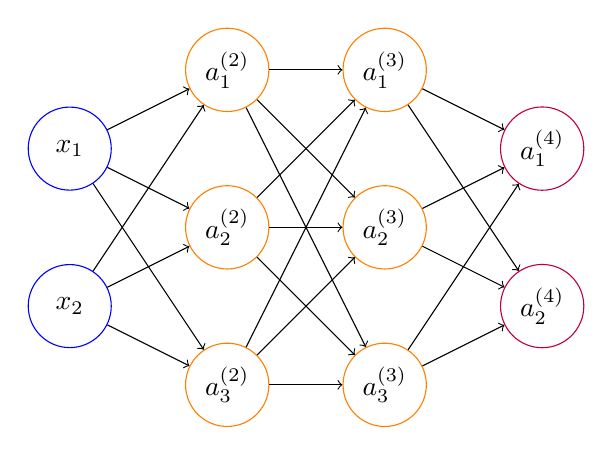
\begin{tikzpicture}
\node[circle,
minimum width =30pt ,
minimum height =30pt ,draw=blue] (1) at(0,2){$x_1$};
\node[circle,
minimum width =30pt ,
minimum height =30pt ,draw=blue] (2) at(0,0){$x_2$};
\node[circle,
minimum width =30pt ,
minimum height =30pt ,draw=orange] (3) at(2,-1){$a_3^{(2)}$};
\node[circle,
minimum width =30pt ,
minimum height =30pt ,draw=orange] (4) at(2,1){$a_2^{(2)}$};
\node[circle,
minimum width =30pt ,
minimum height =30pt ,draw=orange] (5) at(2,3){$a_1^{(2)}$};
\node[circle,
minimum width =30pt ,
minimum height =30pt ,draw=orange] (6) at(4,-1){$a_3^{(3)}$};
\node[circle,
minimum width =30pt ,
minimum height =30pt ,draw=orange] (7) at(4,1){$a_2^{(3)}$};
\node[circle,
minimum width =30pt ,
minimum height =30pt ,draw=orange] (8) at(4,3){$a_1^{(3)}$};
\node[circle,
minimum width =30pt ,
minimum height =30pt ,draw=purple] (9) at(6,2){$a_1^{(4)}$};
\node[circle,
minimum width =30pt ,
minimum height =30pt ,draw=purple] (10) at(6,0){$a_2^{(4)}$};
\draw[->] (1) --(3);
\draw[->] (1) --(4);
\draw[->] (1) --(5);
\draw[->] (2) --(3);
\draw[->] (2) --(4);
\draw[->] (2) --(5);
\draw[->] (3) --(6);
\draw[->] (3) --(7);
\draw[->] (3) --(8);
\draw[->] (4) --(6);
\draw[->] (4) --(7);
\draw[->] (4) --(8);
\draw[->] (5) --(6);
\draw[->] (5) --(7);
\draw[->] (5) --(8);
\draw[->] (6) --(9);
\draw[->] (6) --(10);
\draw[->] (7) --(9);
\draw[->] (7) --(10);
\draw[->] (8) --(9);
\draw[->] (8) --(10);
\end{tikzpicture}
\end{center}
\item bonus:
\begin{center}
\newcommand{\inputnum}{3} 
\newcommand{\hiddennum}{5}  
\newcommand{\outputnum}{2} 
\begin{tikzpicture}
\foreach \i in {1,...,\inputnum}
{
    \node[circle, 
        minimum size = 6mm,
        fill=orange!30] (Input-\i) at (0,-\i) {};
}
\foreach \i in {1,...,\hiddennum}
{
    \node[circle, 
        minimum size = 6mm,
        fill=teal!50,
        yshift=(\hiddennum-\inputnum)*5 mm
    ] (Hidden-\i) at (2.5,-\i) {};
}
\foreach \i in {1,...,\outputnum}
{
    \node[circle, 
        minimum size = 6mm,
        fill=purple!50,
        yshift=(\outputnum-\inputnum)*5 mm
    ] (Output-\i) at (5,-\i) {};
}
\foreach \i in {1,...,\inputnum}
{
    \foreach \j in {1,...,\hiddennum}
    {
        \draw[->, shorten >=1pt] (Input-\i) -- (Hidden-\j);   
    }
}
\foreach \i in {1,...,\hiddennum}
{
    \foreach \j in {1,...,\outputnum}
    {
        \draw[->, shorten >=1pt] (Hidden-\i) -- (Output-\j);
    }
}
\foreach \i in {1,...,\inputnum}
{            
    \draw[<-, shorten <=1pt] (Input-\i) -- ++(-1,0)
        node[left]{$x_{\i}$};
}
\foreach \i in {1,...,\outputnum}
{                \draw[->, shorten <=1pt] (Output-\i) -- ++(1,0)
        node[right]{$y_{\i}$};
}
\end{tikzpicture}
\end{center}
\end{enumerate}
\end{document}
